\documentclass[11pt]{amsart}
\usepackage{geometry}                % See geometry.pdf to learn the layout options. There are lots.
\geometry{letterpaper}                   % ... or a4paper or a5paper or ... 
%\geometry{landscape}                % Activate for for rotated page geometry
%\usepackage[parfill]{parskip}    % Activate to begin paragraphs with an empty line rather than an indent
\usepackage{graphicx}
\usepackage{amssymb,tikz}
\usepackage{epstopdf}
%\usepackage{multicolumn}
\usepackage{tabularx}
\usepackage{subcaption}
\DeclareGraphicsRule{.tif}{png}{.png}{`convert #1 `dirname #1`/`basename #1 .tif`.png}

\title{Methods}
\author{Nick Kappler}


\begin{document}
\begin{figure}
\begin{subfigure}{.45\textwidth}
\caption{Null Model\label{subfig:modelsA}}
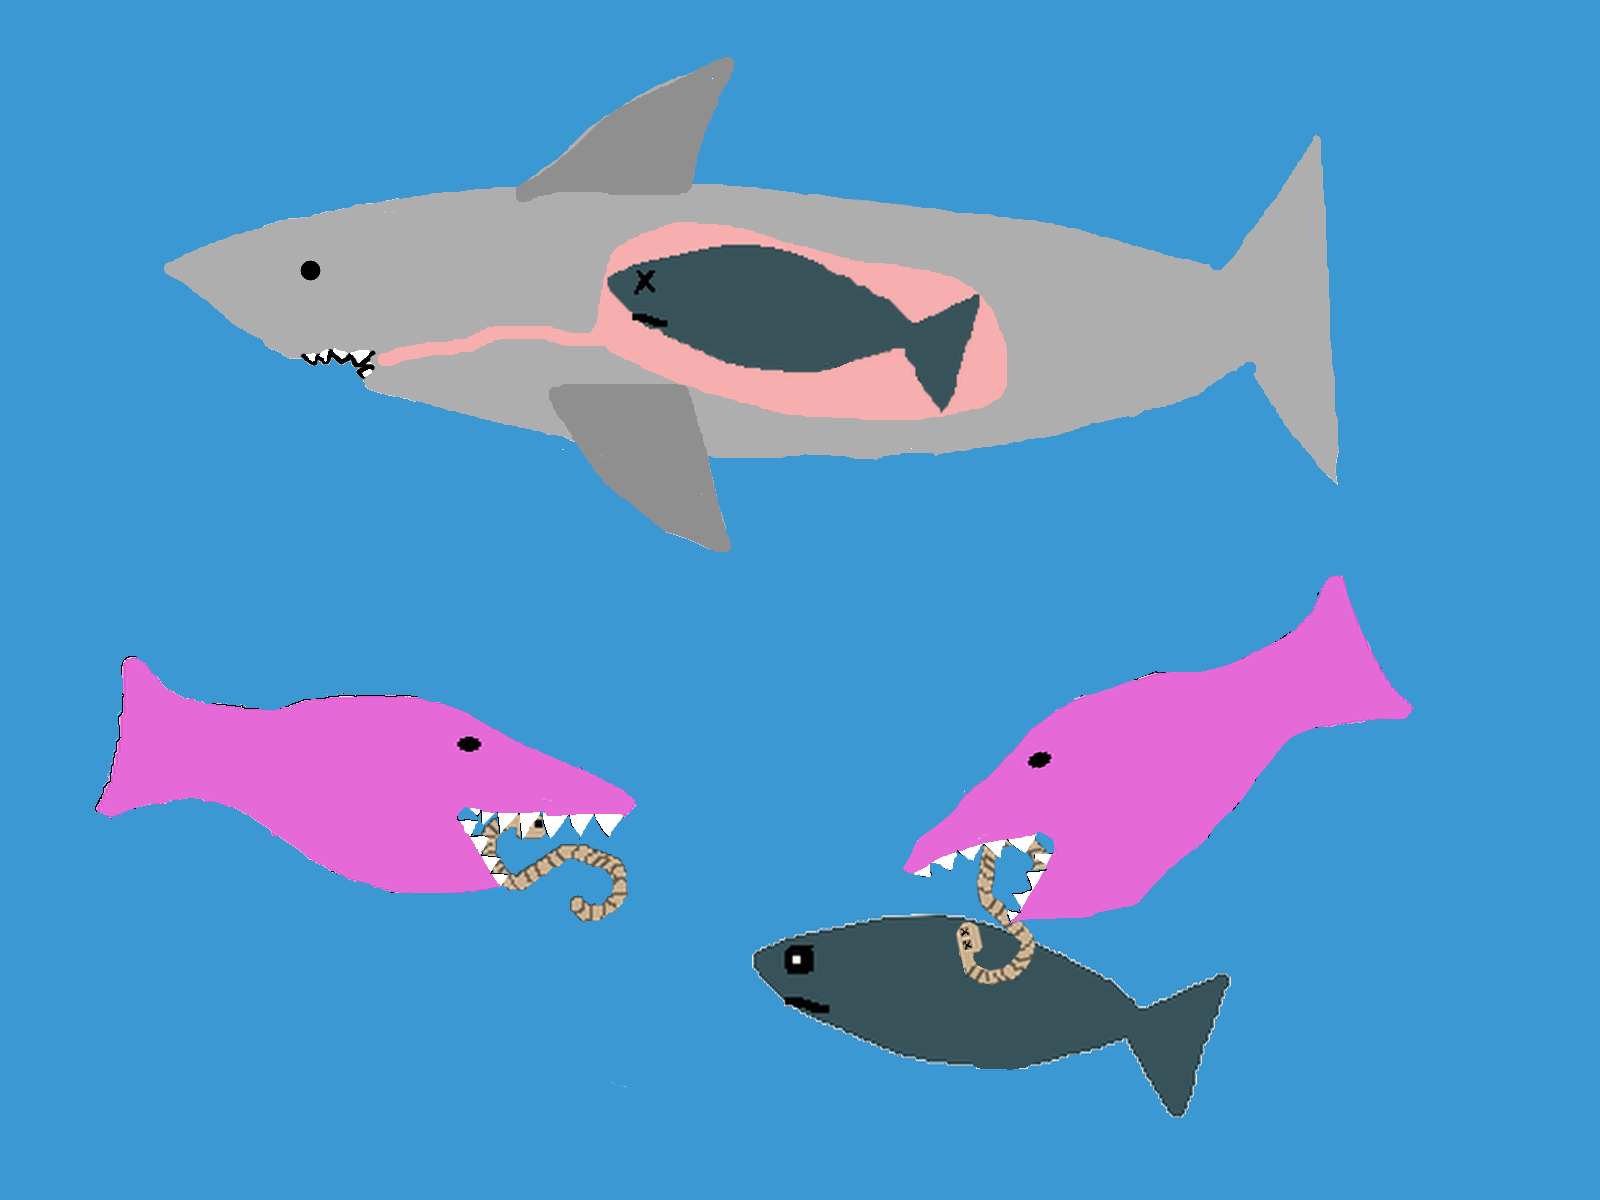
\includegraphics[width=\textwidth]{../figures/Null.png}
\end{subfigure}
\begin{subfigure}{.45\textwidth}
\caption{refuge\label{subfig:modelsB}}
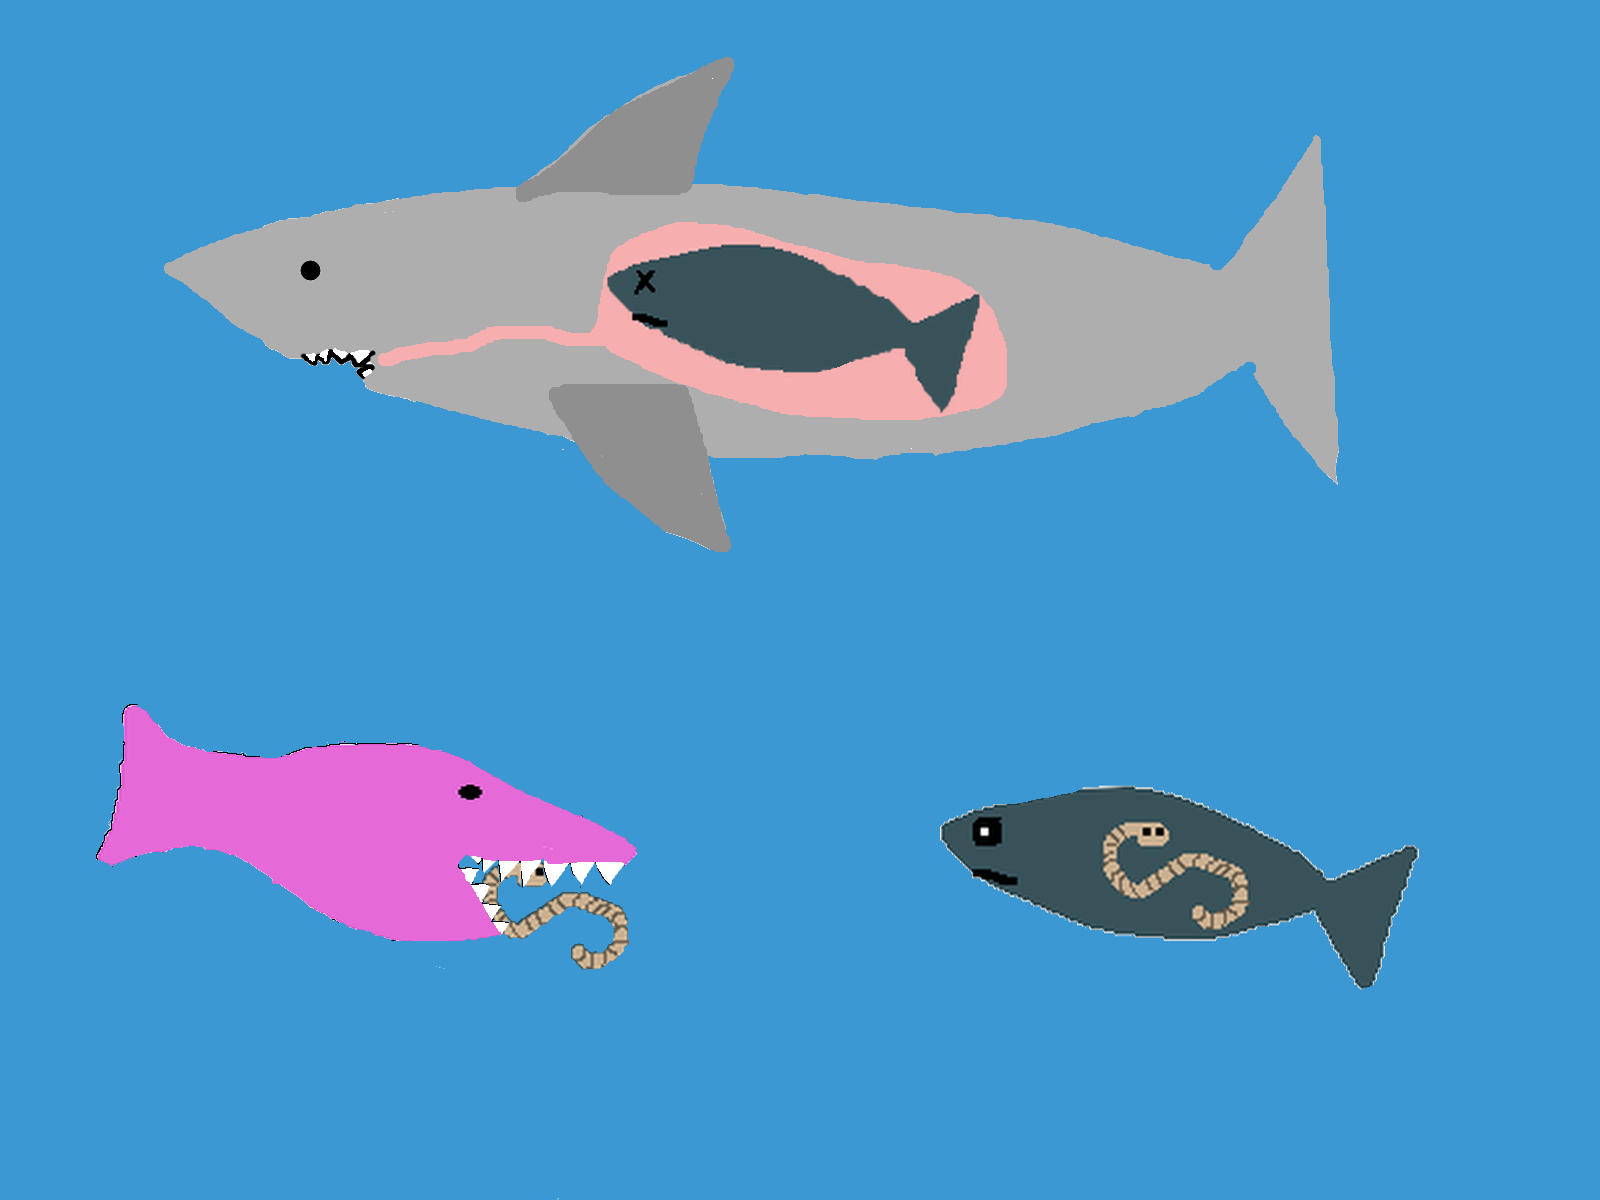
\includegraphics[width=\textwidth]{../figures/Null+Ref.png}
\end{subfigure}

\begin{subfigure}{.45\textwidth}
\caption{concomittant\label{subfig:modelsC}}
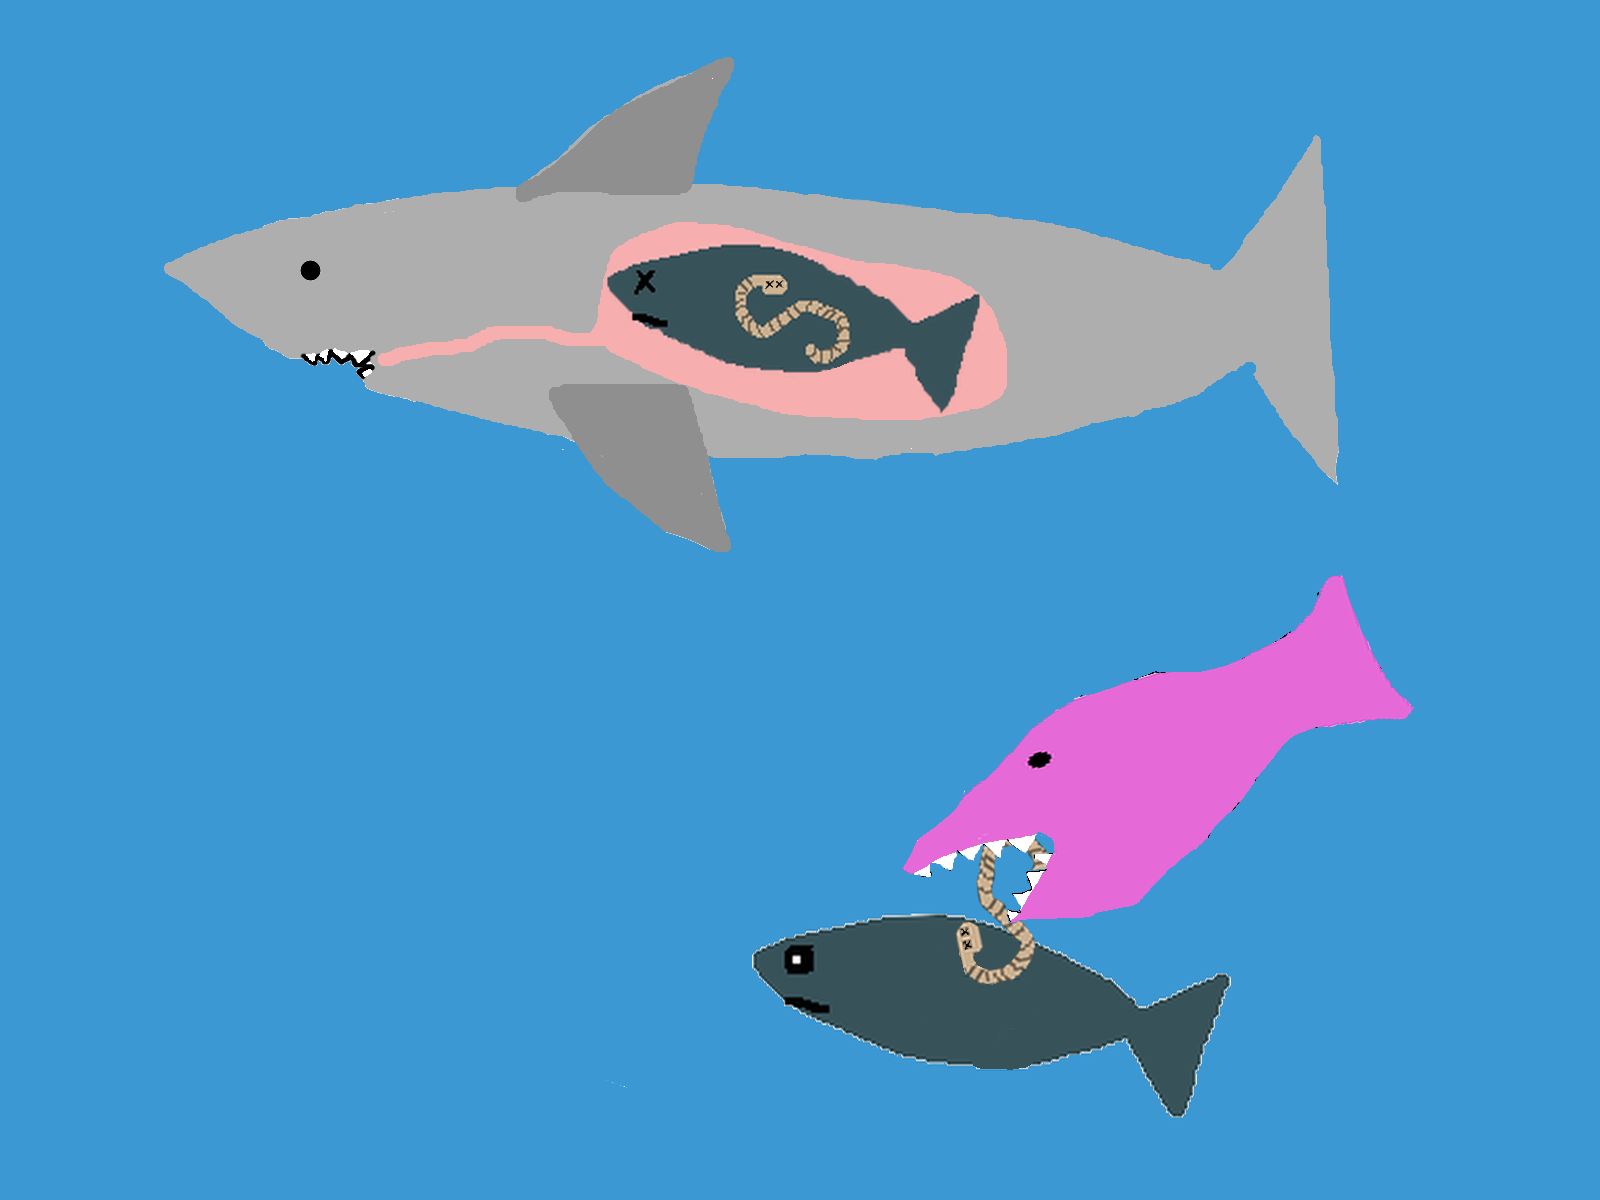
\includegraphics[width=\textwidth]{../figures/Null+Con.png}
\end{subfigure}
\begin{subfigure}{.45\textwidth}
\caption{refuge with concomittant\label{subfig:modelsD}}
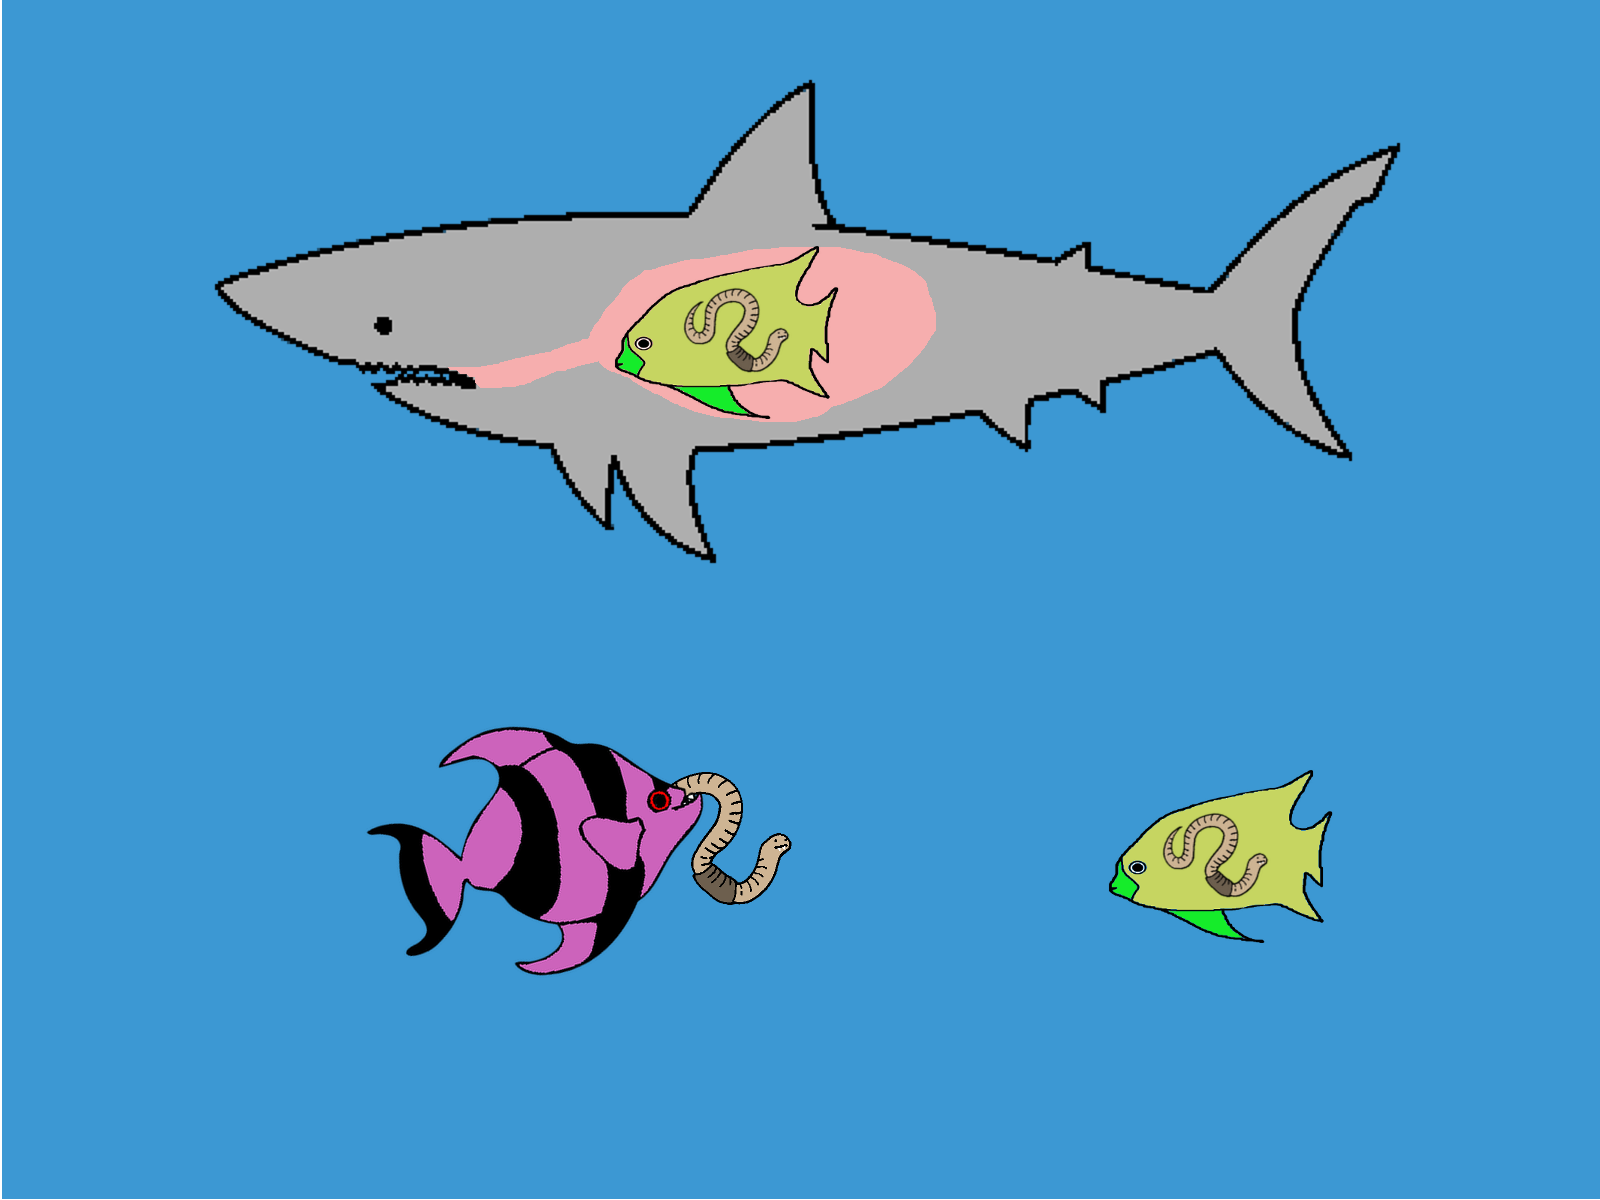
\includegraphics[width=\textwidth]{../figures/Con+Ref.png}
\end{subfigure}
\caption{This cartoon illustrates the differences between the four different versions of ATN dynamics that were tested.  \label{fig:cartoons}}
\end{figure}

In the first model (figure \ref{subfig:modelsA}) parasites are vulnerable to their predators while both inside and outside their hosts and they are not susecptible to concomittant predation.  In this model, the only things that change when a species becomes a parasite are it's body size and metabolic rate.  In the second model, (figure \ref{subfig:modelsB})  we introduce a parameter, $\phi$, to the null model that controls the fraction of parasitic biomass outside of a host at any given time.  A parasite is protected from predation while inside of its host.  However, the parasite is also not susceptible to concomittant predation.  This represents the situation in which parasites are most protected.  The third model (figure \ref{subfig:modelsC}) modifies the null model by making parasites within their hosts susceptible to concomittant predation.  Note that in this model we don't distinguish where a parasite is; so the entire popluation is suscpetible to concomittant predation and normal predation.  This model represents the most vulnerable state for parasites.  In the final model (figure \ref{subfig:modelsD}) we use the parameter $\phi$ to determine what fraction of parasitic biomass is susceptible to concomittant predation.  The fraction of parasitic biomass that is inside a host is protected from standard predation.  This was designed to be the most 'realistic' situation.


\end{document}
